\documentclass[preprint,12pt,authoryear]{elsarticle}

%% Essential Packages
\usepackage{amssymb}
\usepackage{amsmath}
\usepackage{graphicx}
\usepackage[utf8]{inputenc} % Required for accents (ç, ã, é)
\usepackage{booktabs}
\usepackage{lipsum}
\usepackage{url}
\usepackage{algorithm}
\usepackage{algorithmicx}
\usepackage{algpseudocode}

\journal{Expert Systems with Applications} 

\begin{document}

\begin{frontmatter}

%% Title
\title{Enhancing Metaheuristics for Pistachio Supply Chain Optimization}
%title{"A Tailored Variable Neighborhood Search for Large-Scale Pistachio Supply Chain Design"}

%% Authors
%% We map authors to affiliations using labels [aff1, aff2]

\author[aff1]{Raissa Gonçalves Diniz}
\ead{raissagd@ufmg.br}

\author[aff1,aff2]{André Costa Batista}
\ead{andre-costa@ufmg.br}

%% Affiliations

%% Affiliation 1
\affiliation[aff1]{organization={Operations Research and Complex Systems Laboratory, Universidade Federal de Minas Gerais},
            country={Brazil}}

%% Affiliation 2
\affiliation[aff2]{organization={Department of Electrical Engineering, Universidade Federal de Minas Gerais},
            addressline={Av. Antônio Carlos 6627},
            city={Belo Horizonte},
            postcode={31270-010},
            state={Minas Gerais},
            country={Brazil}}

%% Abstract
\begin{abstract}
Efficient supply chain management is critical for high-value agricultural products. While mixed-integer linear programming models for the pistachio industry exist, 
the literature lacks efficient heuristic approaches with clear resolution methodologies. This paper addresses this issue by presenting an enhanced Variable Neighborhood Search (VNS) 
approach. Unlike prior studies that used real-valued encoding with unspecified decoding steps, we propose a transparent integer encoding scheme and a rigorous decoding algorithm. 
Furthermore, we develop domain-specific neighborhood structures that significantly improve search convergence compared to classical operators. We benchmark our method against Genetic 
Algorithms (GA), Iterated Local Search (ILS), and an exact solver. The experiments reveal that while the exact method provide optimal solutions for small instances, the proposed VNS is 
robust and superior in finding high-quality solutions for large-scale datasets, outperforming other metaheuristics in both stability and objective function values.
\end{abstract}

%% Keywords
\begin{keyword}
Supply Chain Optimization \sep Metaheuristics \sep Variable Neighborhood Search \sep Sustainable Logistics
\end{keyword}

\end{frontmatter}

%% Main Text

% ----------------------------------------------------------------------------------------------------------------------
\section{Introduction}
\label{sec:intro}

The growing role of agriculture in the economic development of many countries highlights the importance of integrating this sector with 
other industries to stimulate overall economic growth. Agriculture not only supports food security but also acts as a major contributor 
to exports, generating significant income and strengthening other sectors. Among various agricultural products, pistachios stand out due to 
their high economic and nutritional value. Major producers such as the US, Turkey, and Iran dominate global pistachio production, 
remaining the leading producers worldwide in 2022 and 2023 (\cite{statista2023}). As a result, the strategic importance of pistachios in international trade continues to grow.

With the increasing global demand for pistachios, the need for efficient supply chain networks becomes more critical. Proper supply chain 
management is vital for maintaining product quality, minimizing environmental impacts, and ensuring the smooth flow of goods from production 
to consumers. A key challenge in pistachio production is the management of its by-products, such as hulls and shells, which, while free of heavy 
metals or pathogens, can degrade soil quality and contribute to environmental pollution if not properly handled (\cite{doula2014, bartzas2017}). 
Furthermore, improper disposal of these materials may lead to the growth of molds that increase the risk of aflatoxin contamination, posing serious 
health risks such as liver cancer (\cite{hokmabadi2018,dronavalli2019}). Therefore, eco-friendly practices for reusing agricultural waste are 
essential to mitigate both environmental and health hazards.

Moreover, inefficiencies in supply chain networks for food and agricultural products, including pistachios, can have significant 
implications for product quality and trade (\cite{casper2018}). Addressing these environmental and logistical concerns is crucial to sustaining both 
the economic and ecological viability of the pistachio industry.  In the broader context of sustainable supply chains, several studies have focused on 
optimizing resource use and minimizing waste through recovery and recycling practices. For example, sustainable supply chain models designed for 
agriculture and other industries have shown significant environmental benefits by reducing waste and reusing by-products for processes like 
biogas and compost production (\cite{cheraghalipour2022}). Such approaches have been successfully applied in sectors such as manufacturing 
and waste recovery, where efficient resource management and cost reduction have been key drivers (\cite{devika2014, zohal2016}). 
These strategies underline the importance of sustainability in modern supply chains and the potential for agricultural industries to implement similar measures.

In related research, \cite{rajabi2023} focused on optimizing the pistachio supply chain using various algorithms, primarily population-based 
approaches such as the Genetic Algorithm (GA) (\cite{fathollahi2018, xie2022}), among others. However, a significant limitation in their work is the lack of methodological transparency. 
Specifically, the authors employed a real-valued encoding scheme without detailing the decoding procedure required to transform these values into a feasible transport tree. 
This omission hinders reproducibility and obscures the mechanism by which constraints are handled. Furthermore, the literature has increasingly questioned the effectiveness 
of "metaphor-based" metaheuristics (such as the Imperialist Competitive Algorithm and the Social Engineering Optimizer, used by the authors), suggesting that established methods 
often perform equally well or better without the complexity of novel analogies (\cite{campelo2023, aranha2022}).

Addressing these gaps, this research focuses on designing an optimal supply chain network for pistachios by leveraging the Variable Neighborhood Search (VNS) algorithm (\cite{gendreau2010}). 
While we adopt the same mixed-integer linear programming (MILP) model formulation from \cite{rajabi2023}, we propose a robust overhaul of the resolution methodology. We introduce a transparent 
integer-based priority encoding and provide a step-by-step description of the decoding algorithm, ensuring reproducibility. Furthermore, we develop problem-specific neighborhood 
operators designed to exploit the particular structure of the chain. These specialized operators are contrasted with classical moves to demonstrate their efficacy in exploring the 
solution space.

To validate the proposed approach, we conduct a comprehensive comparative analysis against a Genetic Algorithm (GA), an Iterated Local Search (ILS), and an exact Branch-and-Cut method 
(using the Gurobi solver). Our findings demonstrate that the proposed VNS with specialized operators consistently outperforms the other metaheuristics in terms of solution quality. 
On top of that, we show that for large-scale instances, where exact methods become infeasible due to memory limitations and excessive runtime, the proposed heuristic offers a vital trade-off, 
providing high-quality (and sometimes, even better) feasible solutions efficiently.

The remainder of this paper is organized as follows. Section~\ref{sec:problem-definition} presents the problem definition and the mathematical formulation. Section~\ref{sec:methodology} 
details the heuristic approach, introducing the integer encoding, the specific decoding steps, and the novel domain-specific neighborhood structures. Section~\ref{sec:experiments} 
reports the computational experiments, offering a statistical comparison between VNS, GA, ILS, and the exact solver across varying instance sizes. Finally, Section~\ref{sec:conclusion} 
summarizes the key findings and suggests future research directions.

% ----------------------------------------------------------------------------------------------------------------------
\section{Problem Definition}
\label{sec:problem-definition}

The logistics network proposed by \cite{rajabi2023}, illustrated in Figure~\ref{fig:supplychain}, describes the flow of products and by-products along the pistachio supply chain. 
The process begins with the farmers ($i$), who send the harvested pistachios to the processing centers ($j$). At these centers, the pistachios are transformed into three main components: 
open-shell pistachios, raw kernels, and organic waste.

Each of these components follows specific flows. Open-shell pistachios are forwarded to pistachio factories ($k$), which process and distribute them to final customers ($n_1$). 
Raw kernels are sent to oil extraction centers ($e$), responsible for producing pistachio oil, which is directed to both final customers ($n_2$) and cosmetic factories ($s$). 
These, in turn, process the oil into cosmetic products that are supplied to their respective consumers ($n_3$). Organic waste generated in the initial processing is sent to 
composting centers ($q$), where it is transformed into compost, subsequently distributed to composting customers ($m$).

Although, in practical terms, the produced compost could be reused by the original farmers, establishing a closed-loop system, the adopted mathematical model does not explicitly 
represent this feedback. Instead, compost customers are not directly associated with the inital producers, characterizing an implicit feedback cycle. This approach, already 
adopted in previous works (\hspace{-0.03em}\cite{pishvaee2010,ahmadi2019,banasik2016}), preserves the structural simplicity of the model. However, the inclusion of rigorous 
modeling of this return loop represents a promising direction for future investigations, especially in the context of sustainable supply chains.

\begin{figure}
  \begin{center}
      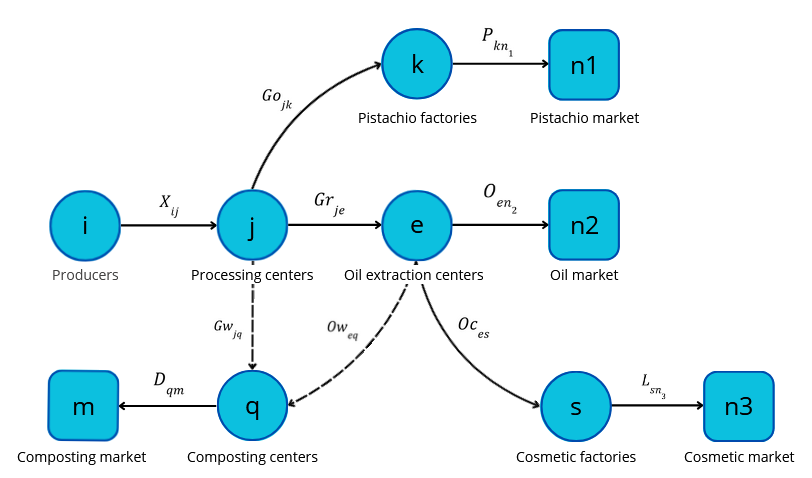
\includegraphics[width=10cm]{./imgs/supplychain.png}
      \caption{Structure of the proposed pistachio supply chain.}
      \label{fig:supplychain}
  \end{center}
\end{figure}

The mixed linear problem aims to minimize total costs \eqref{eq:custo}, including opening, production, and transportation costs, subject to the following capacity and demand constraints, 
tolerating no shortages (see more details on the variables in Table 5 of \cite{rajabi2023}):

\begin{align}
    \min &\ z_1 + z_2 + z_3 \label{eq:custo}\\
    \text{s.t.:} \quad & \sum\limits_{j=1}^J X_{ij} \le Cpa_i, \quad \forall i \in I \label{eq:restricao1}\\
    & \sum\limits_{i=1}^I X_{ij} \le Cpu_j\times U_j, \quad \forall j \in J \label{eq:restricao2}\\
    & \sum\limits_{e=1}^E Ow_{eq} + \sum\limits_{j=1}^J Gw_{jq} \le Cpy_q \times Y_q, \quad \forall q \in Q \label{eq:restricao3} \\
    & \sum\limits_{j=1}^J Go_{jk} \le Cpw_k\times W_k, \quad \forall k \in K \label{eq:restricao4}\\
    & \sum\limits_{j=1}^J Gr_{je} \le Cpr_e\times R_e, \quad \forall e \in E \label{eq:restricao5}\\
    & \sum\limits_{e=1}^E O_{en_2} \le Cpv_s\times V_s, \quad \forall s \in S \label{eq:restricao6}\\
    & \sum\limits_{k=1}^K Go_{jk} + \sum\limits_{e=1} Gr_{je} + \sum\limits_{q=1}^Q Gw_{jq} \le \sum\limits_{i=1} X_{ij}, \quad \forall j \in J \label{eq:restricao7} \\
    & \sum\limits_{k=1}^K Go_{jk} = (1-\beta) \sum\limits_{i=1}^I X_{ij}\theta_1, \quad \forall j\in J \label{eq:restricao8} \\
    & \sum\limits_{e=1}^K Gr_{je} = (1-\beta) \sum\limits_{i=1}^I X_{ij}\theta_2, \quad \forall j\in J \label{eq:restricao9}
\end{align}

\begin{align}
    & \sum\limits_{q=1}^Q Gw_{jq} = \sum\limits_{i=1}^I X_{ij}\theta_3, \quad \forall j\in J \label{eq:restricao10} \\
    & \theta_1 + \theta_2 + \theta_3 = 1 \label{eq:restricao11} \\
    & \sum\limits_{n_1=1}^{N_1} P_{kn_1} \le \sum\limits_{j=1}^J Go_{jk} \times \gamma k, \quad \forall k \in K \label{eq:restricao12} \\
    & \sum\limits_{n_2=1}^{N_2} O_{en_2} + \sum\limits_{s=1}^S Oc_{es} \le \sum\limits_{j=1} Gr_{je}\times(1-\lambda), \quad \forall e\in E \label{eq:restricao13} \\
    & \sum\limits_{q=1}^{Q} Ow_{eq} \le \sum\limits_{j=1}^J Gr_{je} \times \lambda, \quad \forall e \in E \label{eq:restricao14} \\
    & \sum\limits_{n_3=1}^{N_3} L_{sn_1} \le \sum\limits_{e=1}^E Oc_{es} \times \gamma s, \quad \forall s \in S \label{eq:restricao15} \\
    & \sum\limits_{m=1}^M D_{qm} \le \left(\sum\limits_{j=1}^J Gw_{jq} + \sum\limits_{e=1}^E Ow_{eq} \right) \times \gamma q, \quad \forall q \in Q \label{eq:restricao16} \\
    & \sum\limits_{k=1}^K P_{kn_1} \ge Dp_{n_1}, \quad \forall n_1 \in N_1 \label{eq:restricao17}\\
    & \sum\limits_{e=1}^E O_{en_2} \ge Du_{n_2}, \quad \forall n_2 \in N_2 \label{eq:restricao18}\\
    & \sum\limits_{s=1}^S L_{sn_3} \ge Ds_{n_3}, \quad \forall n_3 \in N_3 \label{eq:restricao19}\\
    & \sum\limits_{q=1}^Q D_{qm} \le Dc_{m}, \quad \forall m \in M \label{eq:restricao20}
\end{align}

    
\begin{itemize}
\item The objective function \eqref{eq:custo} minimizes the total costs of the supply chain, including opening, transportation, and production costs. The costs are divided into three components: 
$z_1$ \eqref{eq:custo1}, $z_2$ \eqref{eq:custo2}, and $z_3$ \eqref{eq:custo3}, which represent facility opening costs, transportation costs, and production costs, respectively, as shown in the following equations:
\end{itemize}

\begin{align}
  z_1 &= \sum_{j=1}^J Fu_j \cdot U_j 
      + \sum_{q=1}^Q Fy_q \cdot Y_q 
      + \sum_{k=1}^{K} Fw_k \cdot W_k \notag \\
      &\quad + \sum_{e=1}^{E} Fr_e \cdot R_e
      + \sum_{s=1}^S Fv_s \cdot V_s
      \label{eq:custo1}
\end{align}

\begin{align}
  z_2 &= \sum_{i=1}^I\sum_{j=1}^J CI_i \cdot X_{ij} 
      + \sum_{j=1}^J\sum_{k=1}^K Cu_{1j} \cdot Go_{jk} \notag \\
      &\quad + \sum_{j=1}^J\sum_{e=1}^E Cu_{2j} \cdot Gr_{je} 
      + \sum_{q=1}^Q\sum_{m=1}^M Cy_q \cdot D_{qm} \notag \\
      &\quad + \sum_{k=1}^K\sum_{n_1=1}^{N_1} Cw_k \cdot P_{kn_1} \notag \\
      &\quad + \sum_{e=1}^E Cr_e \cdot \left( \sum_{n_2=1}^{N_2} O_{en_2} 
      + \sum_{s=1}^S Oc_{es} \right) \notag \\
      &\quad + \sum_{s=1}^S\sum_{n_3=1}^{N_3} Cv_s \cdot L_{sn_3}
      \label{eq:custo2}
\end{align}

\begin{align}
  z_3 &= \sum_{i=1}^I\sum_{j=1}^J CX_{ij} \cdot X_{ij} 
      + \sum_{j=1}^J\sum_{k=1}^K CK_{jk} \cdot Go_{jk} \notag \\
      &\quad + \sum_{j=1}^J\sum_{q=1}^Q CJ_{jq} \cdot Gw_{jq}
      + \sum_{e=1}^E\sum_{s=1}^S CS_{es} \cdot Oc_{es} \notag \\
      &\quad + \sum_{e=1}^E\sum_{n_2=1}^{N_2} CN_{en_2} \cdot Oc_{en_2}
      + \sum_{e=1}^E\sum_{q=1}^Q CQ_{eq} \cdot Ow_{eq} \notag \\
      &\quad + \sum_{s=1}^S\sum_{n_3=1}^{N_3} Cl_{sn_3} \cdot L_{sn_3}
      + \sum_{k=1}^K\sum_{n_1=1}^{N_1} Cp_{kn_1} \cdot P_{kn_1} \notag \\
      &\quad + \sum_{q=1}^Q\sum_{m=1}^M Cd_{qm} \cdot D_{qm}
      \label{eq:custo3}
\end{align}

\begin{itemize}
  \item The variables $R_j$, $Y_q$, $W_k$, $Z_e$, and $V_s$ are binary and determine whether certain elements of the model are active. For example, $R_j = 1$ indicates that facility $j$ is 
  operational, and $R_j = 0$ otherwise. The other variables in the model are continuous and non-negative, representing real values greater than or equal to zero. These variables model flows, 
  quantities, and other measurable factors within the system.
  
  \item Constraints \eqref{eq:restricao1}-\eqref{eq:restricao6} address the capacity and demand limitations of each facility in the supply chain. In particular, constraint \eqref{eq:restricao1} 
  limits the quantity of products transported from farmers to distribution centers. Constraints \eqref{eq:restricao2}-\eqref{eq:restricao6} ensure that the quantities sent to processing centers, 
  composting centers, pistachio factories, oil extraction centers, and cosmetic factories do not exceed the capacities of these facilities.
  
  \item The quantity of products shipped from any facility must not exceed the orders received by that facility. Consequently, constraint \eqref{eq:restricao7} establishes that the quantity of 
  products shipped from a processing center must be less than or equal to the quantity received by other facilities. Constraints \eqref{eq:restricao8}-\eqref{eq:restricao11} define the 
  quantities of open-shell pistachios, raw kernels, and waste generated during the hulling process at each processing center. Similarly, constraints \eqref{eq:restricao12}-\eqref{eq:restricao16} 
  govern the flows within pistachio factories, oil extraction centers, cosmetic factories, and composting centers.
  
  \item Finally, to ensure that customer demand is met, constraints \eqref{eq:restricao17}-\eqref{eq:restricao20} ensure that the quantities of products delivered to pistachio, pistachio oil, 
  cosmetics, and compost customers satisfy or exceed their respective demands.
\end{itemize}

% ----------------------------------------------------------------------------------------------------------------------------------------------------------------------------------
\section{Methodology}
\label{sec:methodology}

This section outlines the heuristic methodology employed to solve the optimization problem. The proposed approach integrates a Variable Neighborhood Search (VNS) 
algorithm with a robust priority-based encoding scheme. Our method introduces a transparent integer-based representation and a backward decoding strategy to ensure 
feasibility across the whole chain. Furthermore, to enhance the search capability, we develop and apply problem-specific neighborhood structures designed to exploit the specific 
constraints of the pistachio supply chain.

% ----------------------------------------------------------
\subsection{Solution Representation}
\label{subsec:solution_rep}

Representing a solution for a complex network design problem is non-trivial. Following the principles established by \cite{gen2006} and \cite{rajabi2023}, 
we employ a priority-based encoding method. In this scheme, the chromosome does not directly encode the flow quantities ($X_{ij}$), but rather the \textit{priority} 
of serving specific transportation arcs.

\subsubsection{Integer Permutation vs. Real-Valued Encoding}
In this work, it is used an integer permutation encoding rather than the random key ($0-1$ real value) encoding used in previous studies (\cite{rajabi2023, fathollahi2018}).

In the real-valued approach, genes are assigned random numbers $r \in [0, 1]$, and priorities are derived from sorting these values. This representation suffers from a "many-to-one" 
mapping redundancy: infinite combinations of real numbers can result in the exact same priority order. For example, the vectors $v_1 = [0.1, 0.2, 0.5]$ and $v_2 = [0.8, 0.85, 0.9]$ 
both map to the same permutation indices $(1, 2, 3)$. This redundancy creates "flat" regions in the search landscape where small perturbations (mutations) in the genotype produce no 
change in the phenotype (the solution structure).

In contrast, we employ sequential integers from $1$ to $Z$, where $Z$ is the total number of candidate source-depot pairs in a specific chain segment. This ordinal representation 
ensures a one-to-one mapping between the genotype and the solution structure. This property is crucial for the VNS algorithm, as it ensures that every neighborhood 
move results in a distinct solution configuration, effectively eliminating redundant search steps.

% ----------------------------------------------------------
\subsubsection{Chromosome Structure}
The solution is represented by a composite chromosome divided into eight distinct segments ($S_1$ to $S_8$), as illustrated in Fig. \ref{fig:cromossomo}. Each segment contains a 
permutation of integers representing the transport priorities for a specific part of the supply chain.

\begin{figure}[htbp]
    \centering
    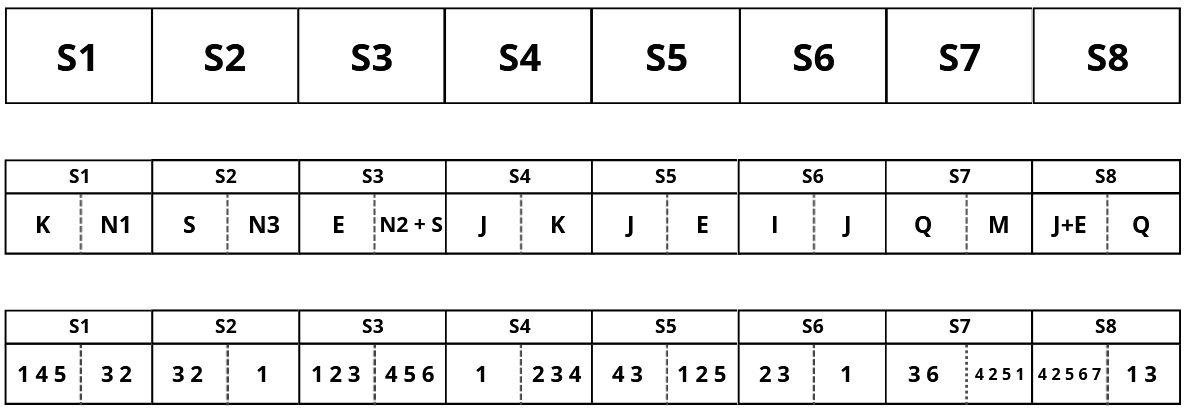
\includegraphics[width=0.8\textwidth]{./imgs/chromo.PNG}
    \caption{Structure of the priority-based chromosome. The solution is composed of 8 distinct integer permutations ($S_1-S_8$), each governing the transport priority of a specific subsection in the supply chain.}
    \label{fig:cromossomo}
\end{figure}

% ----------------------------------------------------------
\subsection{Decoding Procedure}
\label{subsec:decoding}

The decoding process acts as a heuristic builder that transforms the priority chromosome into a feasible transportation tree. As shown in Fig. \ref{fig:decode_flux}, the decoding 
process begins with the flow of final products (pistachios, oil, cosmetics) from factories to consumers. This ensures that all constraints are met: consumer demand is satisfied first, 
propagating the requirements upstream to factories and processing centers, ensuring that facility capacities are respected at every stage.

\begin{figure}[h!]
  \centering
  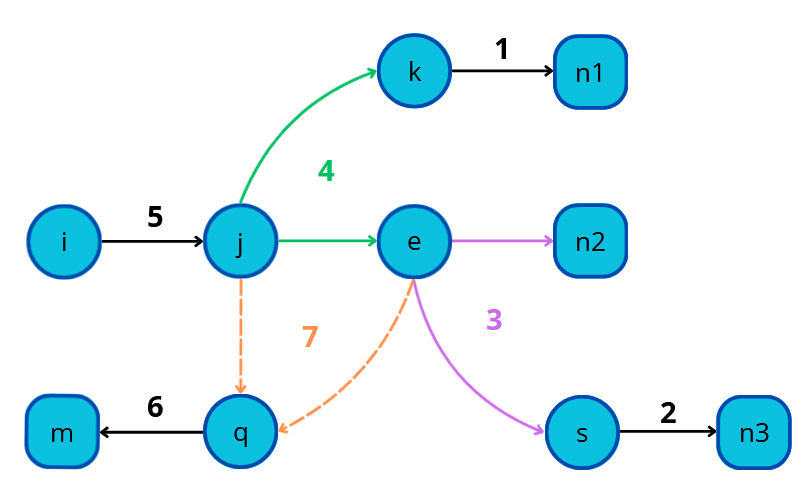
\includegraphics[width=0.9\textwidth]{./imgs/decode_flux.PNG}
  \caption{The backward decoding flow. The process prioritizes satisfying end-consumer demands first to propagate requirements upstream, ensuring feasibility throughout the chain.}
  \label{fig:decode_flux}
\end{figure}

Algorithm \ref{algoDecode1} details the first phase of this process. The procedure utilizes a helper function, \textit{decodingStep}, which implements the classic priority-based 
transportation logic: it allocates flow from sources to destinations based on the priority order defined in the chromosome segment ($S_k$), always selecting the lowest-cost available route.

The critical logic occurs in Steps 5 and 6 (lines 14-17). Here, the algorithm must reconcile the diverging flows from Processing Centers. Since Processing Centers produce multiple 
outputs (Kernels for Oil vs. Open-shell for Factories) in fixed proportions, satisfying the demand of one downstream entity often creates a surplus of the other. Our decoding logic 
identifies the bottleneck demand and routes any inevitable surplus to the destination with the lowest transportation cost, minimizing the penalty for over-supply.

\begin{algorithm}
  \caption{Chromosome decoding for the supply chain (Part 1)}
  \label{algoDecode1}
  \begin{algorithmic}[1]
  \Procedure{Decode}{data}
  \State \textbf{Input:} structured data containing:
  \State - Capacities ($C$) and demands ($D$) for all facilities
  \State - Unit transportation costs ($T$)
  \State - Loss rates for each process stage
  \State - Consumer demands
  \State - Chromosome segments ($S_1, S_2, \ldots, S_8$) representing transport priorities
  \State \textbf{Output:} TotalCost, Decision Variables ($X, P, L, O, \dots$)
  
  \State \textbf{// Step 1: Initialize variables}
  \State $TotalCost \leftarrow 0$

  \State \textbf{// Step 2: Decode Pistachio Factories $\rightarrow$ Pistachio Consumers}
  \State $a_1 \leftarrow$ capacities of pistachio factories
  \State $b_1 \leftarrow$ demands of pistachio consumers
  \State $c_1 \leftarrow$ transportation costs
  \State $(cost1, P) \leftarrow \text{decodingStep}(S_1, a_1, b_1, c_1)$
  \State $TotalCost \leftarrow TotalCost + cost1$
  
  \State \textbf{// Step 3: Decode Cosmetic Factories $\rightarrow$ Cosmetic Consumers}
  \State $a_2 \leftarrow$ capacities of cosmetic factories
  \State $b_2 \leftarrow$ demands of cosmetic consumers
  \State $c_2 \leftarrow$ transportation costs
  \State $(cost2, L) \leftarrow \text{decodingStep}(S_2, a_2, b_2, c_2)$
  \State $TotalCost \leftarrow TotalCost + cost2$
  
  \State \textbf{// Step 4: Decode Oil Extraction Centers $\rightarrow$ Consumers}
  \State $a_3 \leftarrow$ capacities of oil extraction centers
  \State $b_3 \leftarrow$ demands of oil consumers + cosmetic factories
  \State $c_3 \leftarrow$ transportation costs
  \State $(cost3, OO_c) \leftarrow \text{decodingStep}(S_3, a_3, b_3, c_3)$
  \State Separate $OO_c$ into $O$ (oil consumers) and $O_c$ (cosmetic factories)
  \State $TotalCost \leftarrow TotalCost + cost3$
  
  \State \textbf{// Step 5: Decode Processing Center $\rightarrow$ Pistachio Factories}
  \State $a_4 \leftarrow$ capacities of processing centers
  \State $b_4 \leftarrow$ adjusted demands of pistachio factories
  \State $c_4 \leftarrow$ transportation costs
  \State $(\_\_, G_o) \leftarrow \text{decodingStep}(S_4, a_4, b_4, c_4)$
  
  \State \textbf{// Step 6: Decode Processing Center $\rightarrow$ Oil Extraction Centers}
  \State $a_5 \leftarrow$ capacities of processing centers
  \State $b_5 \leftarrow$ adjusted demands of oil extraction centers
  \State $c_5 \leftarrow$ transportation costs
  \State $(\_\_, G_r) \leftarrow \text{decodingStep}(S_5, a_5, b_5, c_5)$
  \EndProcedure
  \end{algorithmic}
\end{algorithm}

Once the intermediate flows are established, the algorithm proceeds to the upstream and waste management stages, as detailed in Algorithm \ref{algoDecode2}.

First, the exact demand for raw pistachios at the Processing Centers is calculated based on the outputs determined in Phase 1 (lines 2-5). Segment $S_6$ is then used to fulfill 
this demand from Farmers. If the aggregate capacity of farmers is insufficient, the solution is marked as infeasible.

Finally, waste management is handled in Steps 9 and 10. The waste generated at Processing and Oil Extraction centers is "pushed" to Composting Centers. Segment $S_8$ 
determines the priority of these flows, directing waste to the Composting Center with available capacity and the lowest associated cost.

\begin{algorithm}
  \caption{Chromosome decoding for the supply chain (Part 2)}
  \label{algoDecode2}
  \begin{algorithmic}[1]
  \Procedure{Decode}{continuation}
  \State \textbf{// Step 7: Adjust demands at Processing Centers}
  \For{each processing center $j$}
      \State Calculate required outputs based on pistachio and oil flows
      \State Update $G_o$ and $G_r$ to match effective capacities
  \EndFor

  \State \textbf{// Step 8: Decode Pistachio Farmers $\rightarrow$ Processing Centers}
  \State $a_6 \leftarrow$ capacities of pistachio farmers
  \State $b_6 \leftarrow$ updated demands at processing centers
  \State $c_6 \leftarrow$ transportation costs
  \State $(cost6, X) \leftarrow \text{decodingStep}(S_6, a_6, b_6, c_6)$
  \State $TotalCost \leftarrow TotalCost + cost6$
    
  \State \textbf{// Step 9: Decode Composting Centers $\rightarrow$ Compost Consumers}
  \State $a_7 \leftarrow$ capacities of composting centers
  \State $b_7 \leftarrow$ demands of compost consumers
  \State $c_7 \leftarrow$ transportation costs
  \State $(cost7, D) \leftarrow \text{decodingStep}(S_7, a_7, b_7, c_7)$
  \State $TotalCost \leftarrow TotalCost + cost7$
    
  \State \textbf{// Step 10: Assign waste flows}
  \State Calculate waste from processing centers ($J$) and Oil Centers ($E$)
  \State $a_8 \leftarrow$ available capacities of composting centers
  \State $b_8 \leftarrow$ waste demands to be disposed
  \State $c_8 \leftarrow$ transportation costs
  \State $(\_\_, O_w) \leftarrow \text{decodingStep}(S_8, a_8, b_8, c_8)$
  \State Update $TotalCost$
    
  \State \textbf{// Step 11: Define binary opening variables}
  \State Set $U, W, R, V, Y = 1$ if corresponding flow $> 0$
  \State Add fixed costs to $TotalCost$
    
  \State \textbf{return} $TotalCost$, Decision Variables, Binary Variables
  \EndProcedure
  \end{algorithmic}
\end{algorithm}

% ----------------------------------------------------------
\subsection{The VNS Algorithm}
\label{subsec:vns}

The proposed algorithm is a hybrid metaheuristic that enhances the standard Variable Neighborhood Search (VNS) (\cite{hansen2010}) by integrating Variable Neighborhood Descent (VND) 
for intensification and a Simulated Annealing (SA) acceptance criterion. This hybridization addresses the limitations of pure descent methods in the highly constrained landscape of the 
pistachio supply chain. The procedure is outlined in Algorithm \ref{algoVNS}.

The intensification phase employs a Variable Neighborhood Descent (VND) strategy rather than a simple local search. In this step, the algorithm iterates sequentially through the 
entire set of neighborhood structures. Whenever an improvement is found with any operator, the search restarts from the first operator, ensuring that the resulting solution is a local 
optimum with respect to all defined neighborhoods.

To prevent stagnation in local optima, we replace the standard deterministic acceptance criterion with a probabilistic Simulated Annealing mechanism. A new solution generated by 
the VND phase is accepted as the current solution if it improves the objective function or, if it is worse, with a probability given by the Boltzmann factor $P = e^{-\Delta / T}$, 
where $\Delta$ is the deterioration in solution quality and $T$ is the current temperature. This allows the search to traverse valleys in the fitness landscape.

Finally, the shaking phase applies a perturbation to the current solution to escape the basin of attraction of the local optimum. The magnitude of this perturbation is adaptive, 
defined in our implementation as $7\%$ of the total decision variables in the chromosome. This ensures that the diversification strength scales appropriately with the problem size. 
The specific operator used for shaking changes cyclically, reseting to the first operator upon a successful acceptance and moves to the next operator if the candidate solution is rejected.

\begin{algorithm}
    \caption{Hybrid VNS with SA Acceptance}
    \label{algoVNS}
    \begin{algorithmic}[1]
    \Require Initial solution $x$, Operators set $\mathcal{N}$, Max evaluations $N_{max}$, Initial Temp $T_0$, Cooling rate $\alpha$
    \State \textbf{Output:} Best solution found $x^*$
    
    \State $x_{curr} \leftarrow x$; \quad $x^* \leftarrow x$
    \State $n_{eval} \leftarrow 1$; \quad $T \leftarrow T_0$
    \State $k \leftarrow 0$ \Comment{Operator index for shaking}

    \While{$n_{eval} < N_{max}$}
        
        \State \textit{// Phase 1: Intensification (VND)}
        \State $x_{new} \leftarrow \text{VND\_LocalSearch}(x_{curr}, \mathcal{N})$ 
        \State Update $n_{eval}$
        
        \State \textit{// Phase 2: Update Global Best}
        \If{$f(x_{new}) < f(x^*)$}
            \State $x^* \leftarrow x_{new}$
        \EndIf

        \State \textit{// Phase 3: Acceptance Criteria (SA)}
        \State $\Delta \leftarrow f(x_{new}) - f(x_{curr})$
        \If{$\Delta \le 0$ \textbf{or} $\text{Random}(0,1) < e^{-\Delta / T}$}
            \State $x_{curr} \leftarrow x_{new}$
            \State $k \leftarrow 0$ \Comment{Reset shaking operator on acceptance}
        \Else
            \State $k \leftarrow (k + 1) \pmod{|\mathcal{N}|}$ \Comment{Next shaking operator}
        \EndIf

        \State \textit{// Phase 4: Perturbation and Cooling}
        \State $T \leftarrow T \times \alpha$
        \State $x_{curr} \leftarrow \text{Shake}(x_{curr}, \mathcal{N}[k])$
        
    \EndWhile
    \end{algorithmic}
\end{algorithm}

% ----------------------------------------------------------
\subsection{Neighborhood Structures}
\label{subsec:neighborhoods}

A critical inefficiency in applying standard permutation operators to priority-based encoding is their "blindness" to the phenotypic state. 
In the greedy decoding process (Algorithm \ref{algoDecode1}), typically only a subset of high-priority nodes is required to satisfy all demands. 
We term these \textbf{Active Nodes} ($\mathcal{A}$), while the remaining unused nodes are \textbf{Inactive} ($\mathcal{I}$). Standard operators 
often swap two Inactive nodes, changing the genotype but resulting in the exact same transportation tree and objective value.

To overcome this redundancy, our implementation explicitly tracks the set of active nodes returned by the decoder and employs four structure-aware 
operators. These operators are designed to either intensify the search within the current topology or diversify it by forcing interactions between 
the active and inactive sets:

\begin{itemize}
    \item \textbf{Active Reversion:} This operator functions as an intensification mechanism. It selects a segment of the chromosome containing multiple 
    nodes from set $\mathcal{A}$ and reverses their priority values. By reordering only the suppliers that are already in use, this move fine-tunes 
    the flow distribution to find lower-cost allocations without necessarily opening new routes or altering the network structure.

    \item \textbf{Inactive-Active Swap:} This is a global diversification operator. It selects one active node ($i \in \mathcal{A}$) and one inactive 
    node ($j \in \mathcal{I}$) at random and exchanges their priorities. This forces a currently used route to be downgraded and a previously unused 
    route to be upgraded, effectively testing global topology changes by bringing new nodes into the solution.

    \item \textbf{Inactive Boost:} This novel problem-specific operator addresses the "starvation" issue common in capacity-constrained problems. 
    A low-cost supplier might be ignored simply because it sits too low in the priority list to be considered before demands are met. This operator 
    selects a random inactive node and assigns it the highest possible priority value in the chromosome. This forces the greedy decoder to 
    maximize flow from this specific node before considering any others, potentially revealing a completely different and superior tree structure.

    \item \textbf{Inactive-Active Exchange two Neighbors (IA-ETN):} This operator provides a "localized" diversification. Instead of a random global 
    swap, it selects an inactive node and swaps it with its nearest active neighbor in terms of chromosome index distance. Unlike the global 
    swap, which can be highly disruptive, this operator explores the "boundary" of the solution, testing if a route that is "almost" good enough 
    (close to the active set) should replace a marginally active route.
\end{itemize}


% ----------------------------------------------------------------------------------------------------------------------
\section{Computational Experiments}
\label{sec:experiments}
\lipsum[9]

% ----------------------------------------------------------------------------------------------------------------------
\section{Conclusion}
\label{sec:conclusion}
\lipsum[10]

% ----------------------------------------------------------------------------------------------------------------------
%% Bibliography
\bibliographystyle{elsarticle-harv}
\bibliography{references}

\end{document}